\documentclass[a4paper,12pt]{article}

\usepackage{graphicx}   % Imágenes
\usepackage{helvet}     % Fuente de letra
\usepackage[hidelinks]{hyperref}   % Tabla de contenido
\usepackage{url}
\usepackage{etoolbox}
\usepackage{setspace}   % Interlineado
\usepackage{geometry}   % Márgenes
\usepackage{tabularx}   % Tablas

% Márgenes
\geometry{
    a4paper,
    left=25mm,
    right=25mm,
    top=25mm,
    bottom=25mm
}

% Eliminar título de la bibliografía
\patchcmd{\thebibliography}{\section*{\refname}}{}{}{}

\onehalfspacing

\renewcommand{\familydefault}{\sfdefault}
\renewcommand{\contentsname}{Tabla de contenidos}

% Configuración de la portada
\begin{document}

\begin{titlepage}
    \centering
    \vspace*{0.5cm}

    % Logo de la universidad
    
\includegraphics[width=1\textwidth]{logo-tec.png}\par\vspace{1cm}

    % Nombre de la universidad
    {\scshape Instituto Tecnológico de Costa Rica\par}
    \vspace{2cm}

    % Título
    {\Huge\bfseries Proyecto \#2: Parser\par}
    \vspace{2cm}

    % Escuela
    {\large Escuela de Ingeniería en Computación\par}

    % Curso
    {\large Compiladores e Intérpretes IC-5701\par}
    \vspace{2cm}

    % Autor
    {\large Alonso Navarro Carrillo, c. 2022236435\par}
    \vspace{0.25cm}
    {\large Carlos Venegas Masis, c. 2022153870 \par}
    \vspace{0.25cm}
    {\large Valeria Gómez Acuña, c. 2022173229 \par}
    \vspace{2cm}

    \vfill

    % Profesor
    {\large Ing. Ericka Marín Schumann\par}

    % Semestre
    {II Semestre 2024\par}
\end{titlepage}

\tableofcontents\newpage

% Introducción
\section*{Introducción}
\addcontentsline{toc}{section}{Introducción}
\begin{flushleft}
	\hspace*{2em} Este proyecto se ubica en la segunda etapa de la creación de un compilador para el lenguaje de programación C, conocida como el Parsing o Análisis Sintáctico. El propósito principal de esta etapa es diseñar y desarrollar un parser que logre identificar como se relacionan los tokens que se obtenidos de la fase de análisis léxico y determinar si estos tokens forman expresiones, sentencias o estructuras válidas para un programa escrito en lenguaje C. Para lograr esto, se utilizaron dos herramientas Java CUP y JFlex, Java CUP permitió definir reglas gramaticales que describen como deben de combinarse los tokens para ser reconocidos por el parser como correctos. Mientras que JFlex fue utilizado en la etapa de análisis Léxico, esta estapa se desarrolló en la primera fase del proyecto. \par
\vspace{1em}
\hspace*{2em} A lo largo de este documento se detalla el proceso de desarrollo 
del scanner, desde la planificación hasta la implementación y evaluación de los
resultados obtenidos. Se describen decisiones técnicas tomadas para garantizar el
correcto funcionamiento del proyecto, así como las estrategias empleadas para la 
solución de los problemas encontrados durante su desarrollo. 

\end{flushleft}

% Estrategia de solución
\section*{Estrategia de solución}
\addcontentsline{toc}{section}{Estrategia de solución}
\begin{flushleft}
    \hspace*{2em} Después de leer detenidamente la documentación 
    de Java CUP, se comenzó a planear y diseñar la manera en que se iba a conectar el Analizador léxico con el Analizador Sintáctico, 
    aquí surguió el primer problema porque para que funcionaran juntos era necesario modificar la estructura del Analizador Léxico, 
    de manera que devolviera al Analizador Sintáctico los tokens ya analizados. Una vez que se logró hacer esta conexión correctamente, 
    se comenzó con el diseño de las producciones, para ello primero se definieron los terminales y no terminales, luego se inició con el diseño de las 
    producciones de cada uno de los no terminales, aquí surgió el segundo problema porque algunas producciones no eran lo suficientemente 
    específicas en su composición, generando errores debido a ambiguedades, para resolver estos problemas el grupo se reunió y se definieron 
    nuevos no terminales que ayudaron a eliminar ambiguedades y también con la factorización de algunas producciones. \par
   \vspace{1em}
    \hspace*{2em} Cuando se tuvieron las producciones listas se hicieron pruebas para verificar que funcionaban correctamente, 
    luego se comenzó con el manejo de errores para esto se implementó un método llamado Syntax Error este método permite 
    manejar los errores de sintaxis para que el parser los detecte y reporte, los errores se definieron como producciones de los 
   no terminales. POr último se realizaron pruebas para verificar que el parser reconoce las reglas gramaticales e identifica todos los errores. \par
    \vspace{1em}
\end{flushleft}

\newpage

% Análisis de resultados
\section*{Análisis de resultados}
\addcontentsline{toc}{section}{Análisis de resultados}
\begin{table}[!ht]
    \centering
    \begin{tabularx}{\textwidth}{|X|X|X|}
        \hline
        Actividad & Porcentaje realizado & Justificación \\ 
        \hline
        Desplegar lista de errores léxicos & 100\% & \\
        \hline
        Desplegar lista de errores sintácticos & 100\% & \\
        \hline
        Evitar desplegar errores sintácticos en cáscada & 50\% & En situaciones muy específicas el parser se puede caer o dar errores poco precisos. Esto debido a complicaciones en la gramática. \\
        \hline
        Implementar las funciones de read and write & 100\% & \\
        \hline
        Declaración de variables, constantes y lista de variables & 100\% & \\
        \hline
        Reconocer la estructura del programa & 100\% & \\
        \hline
        Identificar funciones & 100\% & \\
        \hline
        Analizar expresiones con operadores aritméticos o booleanos & 100\% & \\
        \hline
        Identificar todas las estructuras de control & 100\% & \\
        \hline
        Definir buenos mensajes de error & 80\% & La mayoría de errores están bien definidos, pero si el flujo es erróneo no se obtiene un buen mensaje. \\
        \hline
    \end{tabularx}
\end{table}

% Lecciones aprendidas
\section*{Lecciones aprendidas}
\addcontentsline{toc}{section}{Lecciones aprendidas}
\begin{flushleft}
	\hspace*{2em} Durante el desarrollo del proyecto, el grupo 
pudo observar que en el parser es fundamental definir correctamente 
la gramática y las reglas de producción. La estructura de las reglas 
y el uso adecuado de precedencia y asociatividad permitieron reducir 
conflictos de análisis, como conflictos shift/reduce o reduce/reduce, 
que dificultan el proceso de análisis sintáctico y provocan errores 
de interpretación. Además, organizar adecuadamente las producciones y 
sus alternativas evitó que ciertas estructuras se interpretaran de 
forma ambigua, lo cual agregó robustez al parser al generar una mejor 
comprensión de la jerarquía entre expresiones y bloques de código. \par
\vspace{1em}
\hspace*{2em} Definir mensajes de error claros fue un reto, especialmente 
al manejar errores sintácticos complejos. En muchos casos, el parser debía 
identificar la causa específica de un error (como la falta de un punto y 
coma o el uso incorrecto de una palabra reservada) y generar un mensaje 
informativo que ayudara a identificar el problema en la línea correspondiente. 
Esto fue esencial para mejorar la experiencia del usuario al facilitar la 
corrección de errores en el código fuente. Asimismo, el equipo experimentó 
con la recuperación de errores para continuar el análisis a pesar de 
errores sintácticos, lo cual permitió al parser brindar un reporte de 
múltiples errores en una sola ejecución, aumentando la eficiencia del 
proceso de depuración.\par
\vspace{1em}
\hspace*{2em} Al enfrentarse a estructuras sintácticas complejas como 
anidación de bloques y condiciones, el equipo comprendió la importancia 
de anticipar casos especiales en las reglas de producción. Definir reglas 
claras para estos casos evitó ambigüedades en el análisis y permitió un 
procesamiento más preciso del código fuente. Esto también permitió al parser 
identificar y manejar constructos incompletos o mal formados de manera 
más efectiva, brindando así una base sólida para la interpretación y 
compilación del código.\par
\vspace{1em}

\end{flushleft}

\newpage

% Casos de prueba
\section*{Casos de prueba}
\addcontentsline{toc}{section}{Casos de prueba}
\subsection*{Caso de prueba 1: Errores en Expresiones Aritméticas y Asignación}
\addcontentsline{toc}{subsection}{Casos de prueba 1: Errores en Expresiones Aritméticas y Asignación}
\begin{flushleft}
    \begin{verbatim}
	void testAsignacionAritmetica() {
		int a = 5;
		int b = 10;
		
		// Error: Falta operando después del operador '+'
		int c = a + ;
		
		// Error: Falta operando antes del operador '-'
		int d = - b;
		
		// Error: Operador de asignación en una expresión aritmética
		a + b = c; 
		
		// Error: Uso de variable no declarada en una operación
		int e = a + f;
		
		// Error: Operación aritmética sin un operando válido
		int g = + + b;
		
		// Error: Falta el punto y coma en la asignación
		int h = a + c
		
		// Expresión correcta (para contraste)
		int i = a * b;
	}
    \end{verbatim}
    Errores esperados:
    \begin{itemize}
	\item Error de sintaxis en línea 6: Error en la expresión
	\item Error de sintaxis en línea 9: Falta operando antes de '-'.
	\item Error de sintaxis en línea 12: Error antes de '=' en asignación.
	\item Error de sintaxis en línea 15: Falta el tipo de dato en la declaración.
	\item Error de sintaxis en línea 18: Falta operando antes de '+'.
	\item Error de sintaxis en línea 18: Falta operando antes de '+'.
	\item Error de sintaxis en línea 21: Error en la expresión
    \end{itemize}
    Resultados:
    \begin{verbatim}
	Starting parsing process...
	Error de sintaxis en línea 6: Error en la expresión
	Error de sintaxis en línea 9: Falta operando antes de '-'.
	Error de sintaxis en línea 12: Error antes de '=' en asignación.
	Error de sintaxis en línea 15: Falta el tipo de dato en la declaración.
	Error de sintaxis en línea 18: Falta operando antes de '+'.
	Error de sintaxis en línea 18: Falta operando antes de '+'.
	Error de sintaxis en línea 21: Error en la expresión
    \end{verbatim}
\end{flushleft}

\newpage

\subsection*{Caso de prueba 2: Errores en Estructuras de Control}
\addcontentsline{toc}{subsection}{Casos de prueba 2: Errores de Paréntesis, Puntos y Comas, y Variables No Declaradas}
\begin{flushleft}
    \begin{verbatim}
    void testEstructurasControl() {
    	int x = 5;
    	int y = 10;
    	// Error: Falta paréntesis de cierre en la condición del 'if'
    	if (x < y {
    		x = x + 1;
    	}
    	// Error: Falta paréntesis de apertura en la condición del 'while'
    	while x < y) {
    		y = y - 1;
    	}
    	// Error: Falta llave de apertura en el bloque del 'else'
    	if (x > y) {
    		print(x);
    	} else 
    		print(y);
    	}
    	// Error: Condición en 'if' sin paréntesis alrededor
    	if x == y {
    		x = x * 2;
    	}
    	// Error: Falta el punto y coma al final de la condición del 'while'
    	while (x < y) {
    		x = x + 1
    	}
    	// Expresión correcta (para contraste)
    	if (x != y) {
    		return;
    	} else {
    		return;
    	}
    }
    \end{verbatim}
Errores esperados:
\begin{itemize}
	\item Error de sintaxis en línea 8: Error en el paréntesis de cierre del if.
	\item Error de sintaxis en línea 13: Falta paréntesis de apertura en el while.
	\item Error de sintaxis en línea 20: Error en la llave de apertura del else.
	\item Error de sintaxis en línea 25: Error en los paréntesis de la condición del if.
	\item Error de sintaxis en línea 29: Falta punto y coma.
\end{itemize}
Resultados:
\begin{verbatim}
Starting parsing process...
Error de sintaxis en línea 8: Error en el paréntesis de cierre del if.
Error de sintaxis en línea 13: Falta paréntesis de apertura en el while.
Error de sintaxis en línea 20: Error en la llave de apertura del else.
Error de sintaxis en línea 25: Error en los paréntesis de la condición del if.
Error de sintaxis en línea 29: Falta punto y coma.

\end{verbatim}
\end{flushleft}

\newpage

\subsection*{Caso de prueba 3: Errores en Declaraciones de Variables}
\addcontentsline{toc}{subsection}{Caso de prueba 3: Errores en Declaraciones de Variables}
\begin{flushleft}
	\begin{verbatim}
		// Error: Identificador sin tipo de dato
		y;
		//Declaracion de una variable
		int x;
		// Declaracion correcta de multiples variables constantes
		const int z, t, y, y;
		// Error: Falta punto y coma en la declaración
		int g, h, i, 
		void testDeclaracionesVariables() {
			// Error: Uso incorrecto de 'void' como tipo de dato en una variable
			void variableInvalida;
			// Error: Falta identificador en la declaración
			int ;
			// Error: Declaración incompleta con un tipo de dato y asignación faltante
			const int ; // Falta un identificador o asignación a la variable constante
			// Declaración correcta (para contraste)
			int valorCorrecto = 10;
			char letra = 'A';
		}
	\end{verbatim}
	Errores esperados:
	\begin{itemize}
		\item Error de sintaxis en línea 5: Falta el tipo de dato en la declaración.
		\item Error de sintaxis en línea 11: Falta punto y coma.
		\item Error de sintaxis en línea 16: Una variable no puede ser declarada void.
		\item Error de sintaxis en línea 19: Falta el identificador de la variable en la declaración.
		\item Error de sintaxis en línea 22: Falta el identificador de la variable en la declaración.
	\end{itemize}
	
	Resultados:
	\begin{verbatim}
		Starting parsing process...
		Error de sintaxis en línea 5: Falta el tipo de dato en la declaración.
		Error de sintaxis en línea 11: Falta punto y coma.
		Error de sintaxis en línea 16: Una variable no puede ser declarada void.
		Error de sintaxis en línea 19: Falta el identificador de la variable en la declaración.
		Error de sintaxis en línea 22: Falta el identificador de la variable en la declaración.
	\end{verbatim}
\end{flushleft}

\newpage

\subsection*{Caso de prueba 4: Errores en Ciclos}
\addcontentsline{toc}{subsection}{Caso de prueba 4: Errores en Ciclos}
\begin{flushleft}
	\begin{verbatim}
		void testCiclos() {
			int x = 0;
			
			// Error: Falta punto y coma en la declaración de 'for'
			for (int i = 0 i < 10; i++) { 
				x += i;
			}
			// Error: While vacio
			while () {
				x += 1;
			}
			// Error: Falta paréntesis de cierre en la condición del 'while'
			while (x < 10 {
				x += 1;
			}
			// Error: do while vacio
			do {
				x += 1;
			} while ();
			// Error: for vacio
			for () {
				x += 1;
			}
			// Error: for con una sola expresion
			for (;) {
				x += 1;
			}
			// Error: Falta paréntesis de apertura en la condición del 'do-while'
			do {
				x += 2;
			} while x < 20);
			// Error: Falta punto y coma al final de la condición en 'do-while'
			do {
				x -= 1;
			} while (x > 0)
			// Error: Falta llave de apertura en el bloque del 'for'
			for (int j = 0; j < 5; j++) 
			x += j;
			}
			// Ciclo correcto (para contraste)
			for (int k = 0; k < 5; k++) {
				x += k;
			}
		}
	\end{verbatim}
	Errores esperados:
	\begin{itemize} 
		\item Error de sintaxis en línea 5: Falta punto y coma.
		\item Error de sintaxis en línea 12: Error en la condición del while.
		\item Error de sintaxis en línea 17: Error en el paréntesis de cierre del while.
		\item Error de sintaxis en línea 22: Error en la condición del do-while.
		\item Error de sintaxis en línea 27: Error en la sentencia del for.
		\item Error de sintaxis en línea 30: No puede haber una sola expresión.
		\item Error de sintaxis en línea 37: Falta paréntesis de apertura en el do-while.
		\item Error de sintaxis en línea 42: Falta punto y coma.
		\item Error de sintaxis en línea 47: Error en la llave de apertura del for.
	\end{itemize}
	Resultados:
	\begin{verbatim}
	Starting parsing process...
	Error de sintaxis en línea 5: Falta punto y coma.
	Error de sintaxis en línea 12: Error en la condición del while.
	Error de sintaxis en línea 17: Error en el paréntesis de cierre del while.
	Error de sintaxis en línea 22: Error en la condición del do-while.
	Error de sintaxis en línea 27: Error en la sentencia del for.
	Error de sintaxis en línea 30: No puede haber una sola expresión.
	Error de sintaxis en línea 37: Falta paréntesis de apertura en el do-while.
	Error de sintaxis en línea 42: Falta punto y coma.
	Error de sintaxis en línea 47: Error en la llave de apertura del for.
	\end{verbatim}
\end{flushleft}

\subsection*{Caso de prueba 5: Errores en Funciones y Parámetros}
\addcontentsline{toc}{subsection}{Caso de prueba 5: Errores en Funciones y Parámetros}
\begin{flushleft}
	\begin{verbatim}
		// Error: Falta tipo de retorno en la declaración de la función (No funciona)
		suma(int a, int b) {
			return a + b;
		}
		// Error: Falta identificador en el parámetro de la función
		int resta(int a, ) {
			return a - b;
		}
		// Error: Falta llave de cierre en el cuerpo de la función (Tira Falta punto y coma)
		int multiplica(int a, int b) 
			int resultado = a * b;
			return resultado;
		}
		int dividir int a, int b) {
			return a / b;
		}
		int dividir (int a, int b {
			return a / b;
		}
		void calcularSuma(int a, int b) {
			return a + b;
		}
		// Función correcta (para contraste)
		int modulo(int a, int b) {
			return a % b;
		}
	
	\end{verbatim}
	Errores esperados:
	\begin{itemize} 
	\item Error de sintaxis en línea 2: Falta el tipo de dato en la declaración de la función.
	\item Error de sintaxis en línea 7: Error en la coma de los parametros.
	\item Error de sintaxis en línea 16: Error en las llaves de la función.
	\item Error de sintaxis en línea 18: Error en los paréntesis de la función.
	\item Error de sintaxis en línea 22: Error en la coma de los parametros.
	\end{itemize}

	Resultados:
	\begin{verbatim}
	Starting parsing process...
	Error de sintaxis en línea 2: Falta el tipo de dato en la declaración de la función.
	Error de sintaxis en línea 7: Error en la coma de los parametros.
	Error de sintaxis en línea 16: Error en las llaves de la función.
	Error de sintaxis en línea 18: Error en los paréntesis de la función.
	Error de sintaxis en línea 22: Error en la coma de los parametros.
	\end{verbatim}
\end{flushleft}

\newpage

\subsection*{Caso de prueba 6: General}
\addcontentsline{toc}{subsection}{Caso de prueba 6: General}
\begin{flushleft}
	\begin{verbatim}
		void funcionGeneral() {
			int a = 5;
			int b = 10
			// Error: Declaración de variable con tipo inválido
			void varInvalida = 20;
			// Error: asignación inválida
			a + b = c;
			// Error: Falta paréntesis de cierre en la condición del 'if'
			if (a < b {
				print(a);
			} else {
				print(b)
			}
			// Error: Falta el paréntesis de apertura en el 'while'
			while a < b) {
				a = a + 1;
			}
			// Error: Falta punto y coma en la declaración de 'for'
			for (int i = 0 i < 10; i++) {
				print(i);
			}
			// Error: Paréntesis no cerrado en una expresión aritmética 
			a + (b * 2 ;
			
			// Declaración correcta para contraste
			if (x != a) {
				print("x y a son diferentes");
			}
		}
		
	\end{verbatim}
	Errores esperados:
	\begin{itemize}
	\item	Error de sintaxis en línea 3: Falta punto y coma.
	\item	Error de sintaxis en línea 5: Una variable no puede ser declarada void.
	\item	Error de sintaxis en línea 8: Error antes de '=' en asignación.
	\item	Error de sintaxis en línea 14: Falta punto y coma.
	\item	Error de sintaxis en línea 13: Error en el paréntesis de cierre del if.
	\item	Error de sintaxis en línea 20: Falta paréntesis de apertura en el while.
	\item	Error de sintaxis en línea 23: Falta punto y coma.
	\item	Error de sintaxis en línea 28: Error en paréntesis de expresión.
	\item	Error de sintaxis en línea 33: Error en la llave de apertura del if.
	\end{itemize}
	Resultados:
	\begin{verbatim}
	Starting parsing process...
	Error de sintaxis en línea 3: Falta punto y coma.
	Error de sintaxis en línea 5: Una variable no puede ser declarada void.
	Error de sintaxis en línea 8: Error antes de '=' en asignación.
	Error de sintaxis en línea 14: Falta punto y coma.
	Error de sintaxis en línea 13: Error en el paréntesis de cierre del if.
	Error de sintaxis en línea 20: Falta paréntesis de apertura en el while.
	Error de sintaxis en línea 23: Falta punto y coma.
	Error de sintaxis en línea 28: Error en paréntesis de expresión.
	Error de sintaxis en línea 33: Error en la llave de apertura del if.
	\end{verbatim}
\end{flushleft}

\newpage

% Manual de usuario
\section*{Manual de usuario}
\addcontentsline{toc}{section}{Manual de usuario}
\subsection*{Instalación}
Para construir y ejecutar el proyecto, es necesario tener Java instalado en tu sistema. Sigue estos pasos para configurar el proyecto:

\begin{enumerate}
    \item Clona el repositorio:
    \begin{verbatim}
    git clone https://github.com/AlonsoNav/CCompilerJFlex.git
    cd your-repo
    \end{verbatim}

    \item Genera el archivo \texttt{CLexer}:
    \begin{verbatim}
    java -jar lib/jflex-full-1.9.1.jar src/scanner/CLexer.flex
    \end{verbatim}

	\item Genera el archivo \texttt{Parser}:
	\begin{verbatim}
	java -jar lib/java-cup-11b.jar -parser Parser -symbols Symbol 
	src/parser/Parser.cup
	\end{verbatim}

    \item Compila el proyecto:
    \begin{verbatim}
    javac -d bin -sourcepath src -cp lib/java-cup-11b.jar 
	src/app/ParserMain.java src/app/ScannerMain.java 
	src/scanner/CLexer.java src/scanner/Token.java 
	src/scanner/TokenType.java src/parser/Parser.java 
	src/parser/Sym.java
    \end{verbatim}
\end{enumerate}

\subsection*{Uso}
Para ejecutar el compilador con un archivo de entrada, utiliza el siguiente comando:
\begin{verbatim}
    java -cp bin app.ParserMain input_file
\end{verbatim}

% Bitácora
\section*{Bitácora}
\addcontentsline{toc}{section}{Bitácora}

\subsection*{Fecha: 17-10-2024}
\begin{flushleft}
    \hspace*{2em} Para iniciar el proyecto hicimos una pequeña
    reunión en la que se estableció que CV se encargaba de las
    variables, declaraciones y constantes. Por otro lado, VG
	iba a trabajar las estructuras de control como condicionales
	y bucles. AN diseñaría las gramáticas para las expresiones, 
	y las funciones como read y write. CV también trabajó en la 
	conversión de los tokens del scanners a Symbol y además de dar 
	la estructura básica del programa. A continuación se adjunta 
	evidencia de lo hablado en un chat de WhatsApp:\par\vspace{1em}
	\centering
	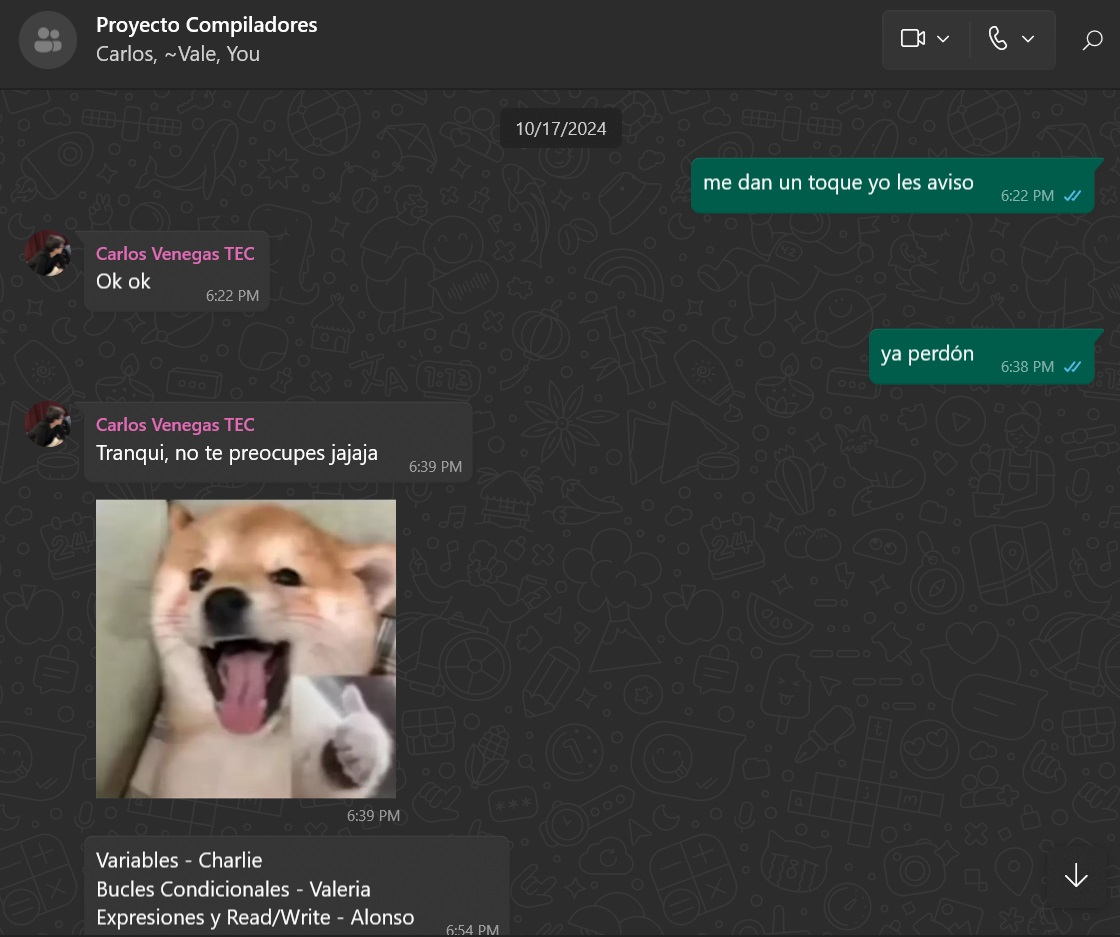
\includegraphics[width=0.5\textwidth]{log_1.jpg}\par
\end{flushleft}

\subsection*{Fecha: 26-10-2024}
\begin{flushleft}
    En este día nos conectamos un rato en Discord para revisar 
	lo que tenemos trabajado hasta el momento y discutir las 
	próximas etapas del proyecto. Para el manejo de errores se hizo 
	otra distribución donde CV se encargaba de errores de expresiones 
	y de read and write, AN de errores de estructuras de control y VG 
	de errores de variables, constantes y funciones.
\end{flushleft}

\subsection*{Fecha: 04-09-2024}
\begin{flushleft}
    \hspace*{2em} Para este punto se tienen muchas complicaciones 
	con el manejo de errores, por lo que a partir de este día se 
	tienen reuniones consecutivas donde se hace trabajo cooperativo 
	con el fin de sacar las funcionalidades. Por último, se divide 
	las partes de la documentación que serán redactadas por todos 
	los miembros del equipo.
\end{flushleft}

% Bibliografía
\newpage
\section*{Bibliografía}
\addcontentsline{toc}{section}{Bibliografía}
\begin{thebibliography}{9}

\bibitem{examplewebsite}
Klein, G., Rowe, S., \& Décamps, R. (marzo de 2023).
\emph{JFlex User’s Manual}.
JFlex Team.
En: \url{https://www.jflex.de/manual.html}.

\bibitem{examplewebsite}
Hudson, S. (julio de 1999).
\emph{CUP User’s Manual}.
Cup.
En: \url{https://www.cs.princeton.edu/~appel/modern/java/CUP/manual.html#intro}.

\end{thebibliography}

\end{document}